
%%%%%%%%%%%%%%%%%%%%%%% file typeinst.tex %%%%%%%%%%%%%%%%%%%%%%%%%
%
% This is the LaTeX source for the instructions to authors using
% the LaTeX document class 'llncs.cls' for contributions to
% the Lecture Notes in Computer Sciences series.
% http://www.springer.com/lncs       Springer Heidelberg 2006/05/04
%
% It may be used as a template for your own input - copy it
% to a new file with a new name and use it as the basis
% for your article.
%
% NB: the document class 'llncs' has its own and detailed documentation, see
% ftp://ftp.springer.de/data/pubftp/pub/tex/latex/llncs/latex2e/llncsdoc.pdf
%
%%%%%%%%%%%%%%%%%%%%%%%%%%%%%%%%%%%%%%%%%%%%%%%%%%%%%%%%%%%%%%%%%%%


\documentclass[runningheads,a4paper]{llncs}

\usepackage{amssymb}
\setcounter{tocdepth}{3}
\usepackage{graphicx}

\usepackage[utf8]{inputenc}
\usepackage[spanish]{babel}

\usepackage{url}
%\urldef{\mailsa}\path|{alfred.hofmann, ursula.barth, ingrid.haas, frank.holzwarth,|
%\urldef{\mailsb}\path|anna.kramer, leonie.kunz, christine.reiss, nicole.sator,|
%\urldef{\mailsc}\path|erika.siebert-cole, peter.strasser, lncs}@springer.com|    
\urldef{\mailsi}\path|siturria,dgarat,gmonce@fing.edu.uy|
\urldef{\nltk}\path|http://www.nltk.org/|
\newcommand{\keywords}[1]{\par\addvspace\baselineskip
\noindent\keywordname\enspace\ignorespaces#1}

\hyphenation{es-tre-cha-men-te in-te-rro-ga-ti-vos in-te-rro-ga-ti-vo he-rra-mien-ta he-rra-mien-tas}

\begin{document}

\mainmatter  % start of an individual contribution

% first the title is needed
\title{Restauración automática de acentos ortográficos en adverbios interrogativos}

% a short form should be given in case it is too long for the running head
\titlerunning{Restauración automática de acentos ortográficos en adverbios interrogativos}

% the name(s) of the author(s) follow(s) next
%
% NB: Chinese authors should write their first names(s) in front of
% their surnames. This ensures that the names appear correctly in
% the running heads and the author index.
%
\author{Santiago Iturriaga \and Diego Garat \and Guillermo Moncecchi} 

%
\authorrunning{Restauración automática de acentos ortográficos en adverbios interrogativos}
% (feature abused for this document to repeat the title also on left hand pages)

% the affiliations are given next; don't give your e-mail address
% unless you accept that it will be published
\institute{Facultad de Ingenier\'ia,\\
Universidad de la Rep\'ublica,\\
Montevideo, Uruguay \\
\mailsi}
%\mailsb\\
%\mailsc\\
%\url{http://www.springer.com/lncs}}

%
% NB: a more complex sample for affiliations and the mapping to the
% corresponding authors can be found in the file "llncs.dem"
% (search for the string "\mainmatter" where a contribution starts).
% "llncs.dem" accompanies the document class "llncs.cls".
%

\toctitle{Lecture Notes in Computer Science}
\tocauthor{Authors' Instructions}
\maketitle

\begin{abstract}
%The abstract goes here. DO NOT USE SPECIAL CHARACTERS, SYMBOLS, OR MATH IN YOUR TITLE OR ABSTRACT.
La omisión de los acentos ortográficos es uno de los errores tipográficos más frecuentes en el idioma español. Su restauración automática consiste en la inserción de acentos   omitidos en los lugares que son necesarios. Los adverbios interrogativos son un caso especialmente dificultoso de este problema, ya que en muchas ocasiones no existen marcas claras que indiquen su presencia. Este trabajo presenta dos técnicas de aprendizaje automático, \emph{Conditional Random Fields} (CRF) y \emph{Support Vector Machines}) aplicadas a la resolución del problema de la restauración automática de acentos ortográficos para el caso específico de los adverbios interrogativos. Se obtuvieron buenos resultados con ambas t\'ecnicas, siendo significativamente superior el resultado obtenido utilizando CRF con una disminuci\'on del error del 31,5\%.
\keywords{aprendizaje automático, crf, svm, restauración automática de acentos ortográficos}
\end{abstract}

\section{Introducción}
Dado un texto sin la presencia de acentos ortográficos, el problema de su  restauración automática consiste en insertar acentos ortográficos en los lugares del texto en el que son requeridos por las normas de acentuación. Los acentos ortográficos son muy importantes para determinar el significado de una oración; sin embargo, es muy común omitir este tipo de signo ortográfico en la escritura informal, e.g. es muy común omitir acentos ortográficos en letras mayúsculas.

La acentuación ortográfica en algunas palabras del idioma español sirve solamente como ayuda a la pronunciación. Sin embargo, en otras palabras la acentuación ortográfica elimina la ambigüedad de una oración. Tomando esto en cuenta, podemos clasificar las palabras con acento ortográfico del idioma español de la siguiente manera\cite{CRANDALL95}:
\begin{enumerate}
\item{Palabras sin ambigüedad}. Existe una única forma correcta de escribir estas palabras, e.g. \emph{acentuación} siempre debe ser escrita con tilde.
\item{Palabras con ambigüedad}. Las palabras pertenecientes a esta clase pueden cambiar su significado dependiendo si son escritas con o sin acentuación ortográfica. Por ejemplo: diferentes conjugaciones del mismo verbo (\emph{canto/cantó, hable/hablé}), sustantivos (\emph{papa/papá, secretaria/secretaría}), etc.
\end{enumerate}

La restauración de acentos ortográficos es trivial para las palabras \emph{sin ambig\"uedad}. Sin embargo, la restauración de acentos ortográficos en las palabras \emph{con ambig\"uedad} requiere examinar el contexto de dicha palabra. 

El problema de la restauración de acentos ortográficos se encuentra estrechamente relacionado con los problemas de desambiguación léxica; involucra aspectos de la desambiguación del significado de una palabra y aspectos del etiquetado gramatical. Esta clase de problemas de desambiguación contiene un grupo de problemas muy similares entre sí, e.g. el problema de restauración de mayúsculas, donde se intenta distinguir entre conceptos semánticos diferentes, e.g. papa (tubérculo) y Papa (obispo de Roma).

La restauración de acentos ortográficos es una problemática que ha sido atacada utilizando diferentes técnicas. Crandall\cite{CRANDALL95} propone un método híbrido combinando un método basado en \emph{Hidden Markov Models}(HMM) y un modelo Bayesiano: utiliza ambos modelos eligiendo, para cada palabra, uno u otro dependiendo de la confianza ofrecida por cada método. Simard\cite{SIMARD98}, para la restauración de acentos ortográficos de textos en francés, también propone un método basado HMM combinado con un análisis morfosintáctico del corpus. Yarowsky\cite{YAROWSKY94,YAROWSKY94-2} experimenta con métodos basados en HMM, clasificadores Bayesianos, y listas de decisión para la restauración de acentos ortográficos de textos en español y francés. Todos estos trabajos basan sus métodos de aprendizaje a nivel de palabras, mientras que Mihalcea\cite{MIHALCEA02} presenta un enfoque innovador al utilizar árboles de decisión a nivel de letras para restaurar acentos ortográficos en idioma rumano. La gran mayoría de estos trabajos reportan un porcentaje de éxito muy elevado, pero debe tenerse en cuenta que el porcentaje de éxito del clasificador de línea base también es muy elevado. Por ejemplo, en el idioma francés aproximadamente el $85\%$ de las palabras no llevan acento ortográfico, y la forma correcta de más de la mitad de las palabras restantes puede deducirse determinísticamente. Esto deja una tasa base de éxito del $95\%$\cite{SIMARD98}.

En este trabajo se presenta la aplicación de dos técnicas de aprendizaje automático, CRF y SVM, para la resolución del problema de restauración automática de acentos ortográficos en adverbios interrogativos. Los adverbios interrogativos tienen una gran dependencia con el contexto en el que aparecen y presentan un problema particularmente difícil de resolver debido a su alto nivel ambigüedad.

El trabajo está organizado de la siguiente forma. En la siguiente sección se presenta una descripción del problema. La sección \ref{sec:CRF} presenta la técnica CRF, la primer técnica aplicada. Luego, en la sección \ref{sec:SVM} es introducido SVM, la segunda técnica que fue aplicada al problema. La discusión del análisis experimental y de los resultados obtenidos es presentada en la sección \ref{sec:Resultados}, mientras que las conclusiones y las posibles líneas de trabajo futuro son presentadas en la sección \ref{sec:Conclusiones}.

\section{Descripción del Problema}
Un adverbio se define de la siguiente forma\cite{RAE}.

\begin{enumerate}
\item{m. \emph{Gram}. Palabra invariable cuya función consiste en complementar la significación del verbo, de un adjetivo, de otro adverbio y de ciertas secuencias. Hay adverbios de lugar, como \emph{aquí, delante, lejos}; de tiempo, como \emph{hoy, mientras, nunca}; de modo, como \emph{bien, despacio, fácilmente}; de cantidad o grado, como \emph{bastante, mucho, muy}; de orden, como \emph{primeramente}; de afirmación, como \emph{sí}; de negación, como \emph{no}; de duda o dubitativos, como \emph{acaso}; de adición, como \emph{además, incluso, también}; de exclusión, como \emph{exclusive, salvo, tampoco}. Algunos pertenecen a varias clases.}
\item{m. \emph{Gram}. Los adverbios \emph{como, cuando, cuanto y donde} pueden funcionar como relativos correspondientes a los adverbios demostrativos \emph{así, según, tal, entonces, ahora, tan, tanto, aquí, allí,} etc.; pueden tener antecedente expreso o implícito; p. ej., \emph{la ciudad donde nací; iré donde tú vayas.}}
\item{m. \emph{Gram}. Pueden también funcionar como interrogativos o exclamativos. ORTOGR. Escr. con acento. \emph{¿Cómo estás? ¡Cuánto lo siento!}}
\end{enumerate}

Los adverbios \emph{como, cuando, cuanto y donde} pueden funcionar de forma interrogativa. Cuando un adverbio es interrogativo debe ser acentuado ortográficamente \emph{cómo, cuándo, cuánto y dónde}. Además, el adverbio interrogativo puede formularse de forma directa o indirecta\cite{VECIANA04}. Un ejemplo de un adverbio interrogativo directo es el siguiente: \emph{¿Adónde os marcháis?}. Una frase similar formulada como adverbio interrogativo indirecto es: \emph{Dime adónde saldréis}. Si bien la existencia de signos de interrogación es un fuerte indicador de la presencia de adverbios interrogativos directos, no existe un indicador claro que marque la presencia de los adverbios interrogativos indirectos. Además, dentro de una frase que contiene un adverbio interrogativo pueden presentarse adverbios no interrogativos, e.g. \emph{Cabe preguntarse entonces, ¿por qué algunas enfermedades de origen vírico, como los catarros o la gripe, pueden sufrirse en repetidas ocasiones?}.

El problema que se ataca en este trabajo es el siguiente: dado un texto del que fueron quitados todos los acentos ortográficos de sus adverbios: \emph{cuándo, cuánto, dónde, cómo, adónde, qué}; se debe clasificar cada palabra del texto en una de las siguientes clases: 
\begin{itemize}
	\item {\texttt{O}}. Toda palabra que no es uno de los adverbios considerados.
	\item {\texttt{SIN\_TILDE}}. Si se trata de un adverbio no interrogativo.
	\item {\texttt{CON\_TILDE}}. Si se trata de un adverbio interrogativo (potencialmente un adverbio exclamativo).
\end{itemize}

A continuación se presentan las dos técnicas de aprendizaje automático aplicadas a la resolución del problema.

\section{Conditional Random Fields (CRF)}
\label{sec:CRF}

Conditional random fields\cite{LAFFERTY01} es un modelo estocástico para el etiquetado y la segmentación de datos secuenciales. Utiliza un modelo que define una probabilidad condicional $p(Y|x)$ sobre secuencias de etiquetas dada la observación de una secuencia particular, $x$. Para etiquetar una nueva secuencia observada $x_*$, el modelo condicional selecciona la etiqueta de la secuencia $y_*$ que maximiza la probabilidad condicional $p(y_*|x_*)$. Un modelo CRF puede representarse como un grafo no dirigido en el que cada vértice representa una variable aleatoria y cada arista indica una dependencia entre las variables de los vértices que conecta. De esta manera, sea $X$ la variable aleatoria que representa las secuencias de observaci\'on, definimos $G=(V,E)$ un grafo no dirigido en el que existe un nodo $v \in V$ por cada variable aleatoria representada por el elemento $Y_v$ de $Y$. 

La estructura del grafo que representa el modelo está dada por un único nodo $X$, que representa la entrada completa, y los nodos que representan los elementos $Y$ forman una cadena de primer orden simple (ver la figura \ref{fig:CRF}).

\begin{figure}[ht]
	\centering
	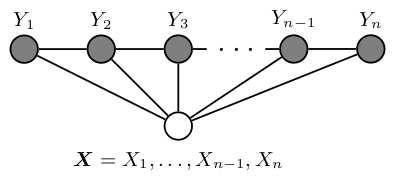
\includegraphics[scale=0.5]{crf.png}
	\caption{Estructura de un modelo CRF.}
	\label{fig:CRF}
\end{figure}

El modelo CRF resulta superior a otros métodos utilizados para el etiquetado de datos secuenciales, como Hidden Markov Model (HMM) o Maximum Entropy Markov Model (MEMM), debido a la relajación en el supuesto de independencia y debido a que evita el problema de sesgo de etiquetado presentados por estos modelos\cite{WALLACH04}.

\section{Support Vector Machines (SVM)}
\label{sec:SVM}

Support vector machines\cite{JOACHIMS99} es un clasificador lineal. Dado una serie de vectores de entrada, SVM intenta dividir linealmente el espacio vectorial creando una serie de regiones, a cada una de las cuales se le asocia una clase de salida. En el caso más simple de dos dimensiones tendremos un conjunto de instancias de entrenamiento ${(x_1, y_1),...,(x_N,y_N)}$, siendo cada instancia $x_i$ un vector en $\Re^N$ y siendo $y_i \in \lbrace-1,+1\rbrace$ la etiqueta de clase correspondiente. El algoritmo SVM aprende un hiperplano lineal que separa el conjunto de ejemplos positivos del conjunto de ejemplos negativos con \emph{margen} máximo. El \emph{margen} se define como la distancia del hiperplano al punto más cercano de cada uno de los conjuntos de ejemplos.

El separador lineal se encuentra definido por un vector de pesos $w$ y un sesgo $b$ que representa la distancia del hiperplano al origen. La regla de clasificación de SVM es entonces $f(x,w,b)=\langle x \cdot w \rangle+b$ (ver la figura \ref{fig:SVM})~\cite{MATA07}.

\begin{figure}[ht]
	\centering
	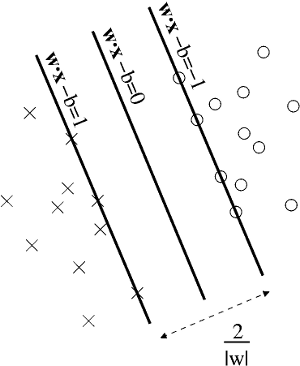
\includegraphics[scale=0.6]{svm.png}
	\caption{Hiperplano que maximiza el margen.}
	\label{fig:SVM}
\end{figure}

\section{Evaluación de las técnicas propuestas}
\label{sec:Resultados}

\subsection{Métricas de Desempeño}
\label{sec:metricas}
Los clasificadores propuestos son evaluados utilizando las métricas de \emph{Precisión}, \emph{Recall} y \emph{Medida-F}. Durante la clasificación de elementos en una clase, el objetivo del clasificador consiste en encontrar la mayor cantidad de elementos de la clase buscada y al mismo tiempo confundir la menor cantidad de elementos de otras clases con los elementos de la clase buscada. La primera parte del objetivo anterior corresponde al concepto de \emph{Recall}, mientras que la segunda parte corresponde al concepto de \emph{Precisi\'on}.

Generalmente las métricas de \emph{Precisión} y \emph{Recall} resultan en conflicto en el sentido de que cuando se intenta aumentar la cantidad de elementos hallados de una clase en particular (i.e. aumentar el \emph{Recall}), usualmente se incrementa también la cantidad de errores cometidos al confundir elementos de otras clases (i.e. disminuye la \emph{Precisión})~\cite{RAGHAVAN89}.

Para definir totalmente las métricas de \emph{Precisión} y \emph{Recall} debemos antes definir los siguientes conceptos.
\begin{itemize}
\item{\emph{Positivos Verdaderos} (PV) son elementos de la clase buscada que fueron correctamente identificados.}
\item{\emph{Negativos Verdaderos} (NV) son elementos que no pertenecen a la clase buscada que fueron correctamente ignorados y clasificados en una clase diferente.}
\item{\emph{Falsos Positivos} (FP), o errores de Tipo I, son elementos que pertenecen a otra clase y que fueron incorrectamente clasificados en la clase buscada.}
\item{\emph{Falsos Negativos} (FN), o errores de Tipo II, son elementos que pertenecen a clase buscada y que fueron incorrectamente clasificados en otra clase.}
\end{itemize}

En base a estos conceptos podemos formular matemáticamente la métrica de \emph{Precisión} como se muestra en la ecuación~\ref{eq:precision} y la métrica de \emph{Recall} como se muestra en la ecuación~\ref{eq:recall}~\cite{BIRD09}.

\begin{equation}
	\label{eq:precision}
	P = \frac{PV}{PV + FP}
\end{equation}
\begin{equation}
	\label{eq:recall}
	R = \frac{PV}{PV + FN}
\end{equation}

La Medida-F combina \emph{Precisi\'on} y \emph{Recall} para obtener una \'unica m\'etrica definida como la media arm\'onica ponderada de \emph{Precisi\'on} y \emph{Recall}. En su formulaci\'on m\'as general, la Medida-F puede expresarse como se presenta en la ecuaci\'on~\ref{eq:medida-f}.

\begin{equation}
	\label{eq:medida-f}
	F_{\alpha} = \frac{P \times R}{(1 - \alpha)P + (\alpha)R}
\end{equation}

Generalmente se utiliza un valor de $\alpha=0.5$ por lo tanto la ecuación~\ref{eq:medida-f} se reduce a la ecuación~\ref{eq:medida-f-0-5}\cite{MAKHOUL99}.

\begin{equation}
	\label{eq:medida-f-0-5}
	F_{0.5} = \frac{2 \times P \times R}{P + R}
\end{equation}

\subsection{Corpus Considerado}
Para la evaluación de las técnicas elegidas se construye un corpus sobre el cual se realiza el entrenamiento y la validación de los clasificadores,  en base a la unión de los corpus CESS Treebanks y CoNLL 2002. Para la construcción del corpus se utiliza la herramienta Natural Languaje Toolkit (NLTK) 2.0~\footnote{Disponible para descargar en \nltk}. Ambos corpus se encuentran incluidos y tokenizados en la herramienta NLTK, por lo tanto la utilización de NLTK facilita la construcción del corpus de trabajo.

El corpus construido consta de un total de $562136$ tokens, de los cuales $18677$ son adverbios no interrogativos y $238$ son adverbios interrogativos. En el cuadro \ref{table:corpus} se muestra la proporci\'on de las etiquetas asignas al corpus construido.

%Aprox. 74 de 238 adeverbios interrogativos directos. El resto son indirectos. ¿31%?

\begin{table}[ht]
 	\renewcommand{\arraystretch}{1.3}
	\renewcommand{\tabcolsep}{3pt}
	\caption{Etiquetas asignadas al corpus utilizado.}
	\label{table:corpus}
	\centering
	\begin{tabular}{c r r}
		\hline\hline
		\multicolumn{1}{c}{\textbf{Etiqueta}} & \multicolumn{1}{c}{\textbf{Cantidad de tokens}} & \multicolumn{1}{c}{\textbf{Proporci\'on del corpus}} \\
		\hline
		\texttt{O} & 543221 & 96,64\% \\
		\texttt{SIN\_TILDE} & 18677 & 3,32\% \\
		\texttt{CON\_TILDE} & 238 & 0,04\% \\
		\hline
	\end{tabular}
\end{table}

La gran mayoría de los tokens del corpus (un $96,64\%$)  no son adverbios, y por lo tanto se les asigna la etiqueta \texttt{\small O}. Esto nos asegura que utilizando un clasificador de línea base muy simple podemos obtener fácilmente un $96,64\%$ de precisión asignando la etiqueta \texttt{\small O} a todos los tokens de nuestro corpus. A\'un m\'as, resulta trivial determinar si un token es un adverbio del tipo buscado, por lo tanto basta con asignar la etiqueta \texttt{\small SIN\_TILDE} a todos los adverbios considerados para clasificar correctamente el $98,70\%$ de los adverbios y obtener un $99,96\%$ de \'exito en nuestro clasificador.

\subsection{Herramientas de Implementación}
El clasificador basado en CRF es implementado  utilizando la herramienta MALLET 2.0.6, desarrollada por Andrew McCallum et al.\cite{MCCALLUM02}. MALLET se encuentra implementado en lenguaje Java y se utiliza para el etiquetado de secuencias.

Para la implementaci\'on del clasificador basado en SVM se utiliza SVM$^{light}$, desarrollada en lenguaje C por Thorsten Joachims\cite{JOACHIMS08}. Junto con SVM$^{light}$ se utiliza SVMTool, herramienta desarrollada por el grupo de Procesamiento de Lenguaje Natural de la Universidad Politécnica de Cataluña\cite{GIMENEZ04}\cite{GIMENEZ06}. SVMTool es un generador de etiquetadores de secuencias para SVM$^{light}$ implementado en lenguaje Perl, y permite  la utilizaci\'on de SVM$^{light}$ en problemas de etiquetado de secuencias. 

\subsection{Clasificación Utilizando CRF}
Como ya fue mencionado, se utiliza MALLET para la clasificación mediante CRF. Para definir las características de clasificación, MALLET provee un conjunto de \emph{tubos} que pueden ser aplicados a los tokens del corpus para generar las características deseadas para la clasificaci\'on. Estos \emph{tubos} permiten analizar los tokens mediante expresiones regulares, determinar la posición del token en la oración, obtener subconjuntos de caracteres del token, realizar conjunciones de características de diferentes tokens, etc.

La mayoría de las características utilizadas para la clasificación se especifican con el conjunto de \emph{tubos} incluidos en MALLET, sin embargo para un pequeño conjunto de características es necesario implementar \emph{tubos} adicionales.

En el cuadro \ref{table:featuresCRF} se muestran las características utilizadas para la clasificación mediante CRF.

\begin{table}[ht]
 	\renewcommand{\arraystretch}{1.3}
	\renewcommand{\tabcolsep}{3pt}
	\caption{Características utilizadas para la clasificación mediante CRF.}
	\label{table:featuresCRF}
	\centering
	\begin{tabular}{c l}
		\hline\hline
		\multicolumn{1}{c}{\textbf{Característica}} & \multicolumn{1}{c}{\textbf{Descripción}} \\
		\hline
		\texttt{ADVERBIO} & Tokens que son adverbios. \\
		\texttt{NOADVERBIO} & Tokens que no son adverbios. \\
		\texttt{CAPITALIZED} & Tokens cuya primera letra es mayúscula. \\
		\texttt{FIRST} & Tokens que aparecen primeros en una oración. \\
		\texttt{BEGINNING} & Adverbios que aparecen en primer o segundo lugar \\
		& en una oración. \\
		\texttt{SIGN-QE} & Tokens que representan signos de exclamación. \\
		\texttt{IN-QE} & Adverbios en oraciones donde existen ocurrencias \\
		& de signos de interrogación o exclamación. \\
		\texttt{ADVERBIO-QE} & Adverbios seguidos o precedidos por un signo \\
		& interrogativo o exclamativo. \\
		\texttt{PREV-SINT} & Los siguientes tokens $\rightarrow$ \emph{,} \emph{lo} \emph{la} \emph{el} \emph{los} \emph{"} \\
		\texttt{NEXT-SINT} & Los siguientes tokens $\rightarrow$ \emph{el} \emph{la} \emph{los} \emph{en} \emph{las} \emph{ha} \emph{"} \\
		\texttt{ADVERBIO-SINT} & Adverbios precedidos por \texttt{PREV-SINT} o \\
		& sucedidos por \texttt{NEXT-SINT}. \\
		\texttt{PREV-CINT} & Los siguientes tokens $\rightarrow$ \emph{por} \emph{-} \emph{sobre} \emph{ver} \emph{a} \emph{saber} \emph{sé} \\
		\texttt{NEXT-CINT} & Los siguientes tokens $\rightarrow$ \emph{es} \emph{le} \emph{significa} \\
		\texttt{ADVERBIO-CINT} & Adverbios precedidos por \texttt{PREV-CINT} o \\
		& sucedidos por \texttt{NEXT-CINT}. \\
		\emph{Conjunciones} & Conjunción de todas las características del token anterior \\
		& y el token actual, y todas las características del token \\
		& actual y el token siguiente. \\
		\hline
	\end{tabular}
\end{table}

Las características \texttt{\small PREV-SINT}, \texttt{\small NEXT-SINT}, \texttt{\small PREV-CONT} y \texttt{\small NEXT-CONT} se incluyen luego de realizar un estudio sobre los tokens que preceden y  suceden a los adverbios interrogativos y no interrogativos en el corpus. Existen tokens que preceden o suceden a un adverbio que tienen una gran cantidad de ocurrencias sin importar si el adverbio es interrogativo o no. Sin embargo, otros tokens ocurren (en su mayoría) en el contexto de adverbios interrogativos o adverbios no interrogativos, pero no en ambos.

Se agrega, además, la característica \texttt{\small PREV-SINT} a los tokens que preceden, con mayor ocurrencia, a adverbios no interrogativos y que a su vez no preceden a adverbios interrogativos. De la misma manera se agregan la característica \texttt{\small NEXT-SINT} a los tokens que suceden, con mayor frecuencia, a adverbio no interrogativo, pero no suceden a adverbios interrogativos, y  las características \texttt{\small PREV-CONT} y \texttt{\small NEXT-CONT} para los token que preceden y suceden a adverbios interrogativos, pero no lo hacen con adverbios no interrogativos.

Para el entrenamiento se utiliza un modelo CRF de orden-1 totalmente conectado, optimizando la verosimilitud por etiqueta. Adicionalmente, se prohibe la transición de etiquetas \texttt{\small CON\_TILDE} a \texttt{\small CON\_TILDE} ya que no pueden ocurrir dos adverbios interrogativos juntos en una oración. 

\subsection{Clasificación Utilizando SVM}
Para la clasificación mediante SVM se utiliza la herramienta SVMTool. Se ha aplicado SVMTool a problemas de etiquetado gramatical en español e ingl\'es, logrando en español un porcentaje de éxito en la clasificación del $96,89\%$\cite{GIMENEZ04}. Por defecto, la herramienta SVMTool utiliza para la clasificación las características definidas y optimizadas por Giménez et al.\cite{GIMENEZ04}. En este trabajo se toman como base las caracter\'isticas defecto, calibradas para mejorar su desempeño en el problema de restauración de acentos ortográficos.

En el cuadro \ref{table:featuresSVM} se presentan las características de SVMTool utilizadas para la clasificación.

\begin{table}[ht]
 	\renewcommand{\arraystretch}{1.3}
	\renewcommand{\tabcolsep}{3pt}
	\caption{Características utilizadas en el clasificador SVM.}
	\label{table:featuresSVM}
	\centering
	\begin{tabular}{c l}
		\hline\hline
		\multicolumn{1}{c}{\textbf{Característica}} & \multicolumn{1}{c}{\textbf{Descripción}} \\
		\hline
		\texttt{Tokens} & $t_{-2}$, $t_{-1}$, $t_{0}$, $t_{+1}$, $t_{+2}$ \\
		\texttt{Etiquetas} &  $e_{-2}$, $e_{-1}$ \\
		\texttt{Bigramas$_{t}$} & $(t_{-2},t_{-1})$, $(t_{-1},t_{0})$, $(t_{-1},t_{+1})$, \\
			& $(t_{0},t_{+1})$, $(t_{+1},t_{+2})$ \\
		\texttt{Bigramas$_{e}$} & $(e_{-2},e_{-1})$, $(e_{-1},a_{+1})$, $(a_{+1},a_{+2})$ \\
		\texttt{Trigramas$_{t}$} & $(t_{-2},t_{-1},t_{0})$, $(t_{-2},t_{-1},t_{+1})$, \\
			& $(t_{-1},t_{0},t_{+1})$, $(t_{-1},t_{+1},t_{+2})$, \\
			& $(t_{0},t_{+1},t_{+2})$ \\
		\texttt{Trigramas$_{e}$} & $(e_{-2},e_{-1},a_{+1})$, $(e_{-1},a_{+1},a_{+2})$ \\
		\texttt{SA} & Tokens cuya primera letra es mayúscula. \\
		\texttt{aa} & Tokens en los que todas sus letras son minúsculas. \\
		\texttt{Oraci\'on} & Puntuación de la oración $\rightarrow$ \emph{.} \emph{?} \emph{!} \\
		\hline
	\end{tabular}
\end{table}

Para la clasificación se utiliza una ventana de $5$ tokens centrada en el token a etiquetar. Así $t_{0}$ representa el token a ser etiquetado, $t_{+1}$ el token que sucede a $t_{0}$ en la oración, y $t_{-1}$ el token que lo precede. La característica \texttt{\small Tokens} representa los unigramas formados por los tokens de la oración. De forma similar la característica \texttt{\small Etiquetas} representa las etiquetas de los tokens en la oración; esta característica toma en cuenta las etiquetas de los dos tokens inmediatamente anteriores al token actual.

Adem\'as de los unigramas, para la clasificaci\'on se toman en cuenta bigramas y trigramas tanto de tokens (i.e. \texttt{\small Bigramas$_{t}$}, \texttt{\small Trigramas$_{t}$}) como de etiquetas (i.e. \texttt{\small Bigramas$_{e}$} y \texttt{\small Trigramas$_{e}$}). Para el caso de los bigramas y trigramas de etiquetas ocurre una situaci\'on particular, para formar algunos ngramas se utilizan etiquetas de tokens que se encuentran a la derecha del token que está siendo etiquetado, es decir, etiquetas que aún no han sido asignadas. Existen diferentes formas de resolver este problema, Nakagawa et al.\cite{NAKAGAWA01} propone realizar un etiquetado en dos pasadas para conocer las etiquetas a izquierda y derecha de cada token. La herramienta SVMTool implementa la solución propuesta por Daelemans et al.\cite{DAELEMANS96} que consiste en utilizar etiquetas de ambig\"uedad que representan las posibles etiquetas de los tokens no clasificados.

Las caracter\'istica \texttt{\small Oraci\'on} representa información de puntuación de la oración, e.g. si la oración finaliza con el token \emph{'.'}, o \emph{'?'}, o \emph{'!'}.

En SVMTool existen diferentes modelos para realizar el entrenamiento del clasificador. En este trabajo se utiliza el \emph{Modelo 0} de SVMTool con dos pasadas combinadas (\texttt{\small LRL}). Tal como lo mencionamos antes, en el \emph{Modelo 0} se consideran clases de ambig\"uedad para el contexto desconocido. En un entrenamiento de dos pasadas primero se realiza un entrenamiento de izquierda a derecha (\texttt{\small LR}) y luego de derecha a izquierda (\texttt{\small RL}). Al momento de la clasificación ambas direcciones son evaluadas y es elegida la etiqueta que presenta mayor confiabilidad.

Por último, en SVMTool existen dos posibles esquemas de clasificación, el esquema \emph{Goloso} y el esquema \emph{Por oración}. En el esquema \emph{Goloso} a cada token le es asignada la etiqueta que maximiza la función de puntuación del propio token. En el esquema \emph{Por oración} a cada token le es asignada la etiqueta que maximiza la sumatoria de las funciones de puntuación de todos los tokens de la oración. Se realizaron experimentos con ambos esquemas de clasificación y el esquema \emph{Por oración} arrojó mejores resultados por lo que se decidió utilizar este esquema.

\subsection{Resultados Experimentales}
La plataforma de hardware utilizada para los experimentos consiste en un computador con procesador Intel i3 de 2,13 GHz y 4 GB de RAM. Para la evaluación de los clasificadores se dividió el corpus por oraciones en $10$ partes de tamaño similar; en el cuadro \ref{table:partes-corpus} pueden verse en detalle cada una de las partes. 

\begin{table}[ht]
 	\renewcommand{\arraystretch}{1.3}
	\renewcommand{\tabcolsep}{3pt}
	\caption{Partes del corpus.}
	\label{table:partes-corpus}
	\centering
	\begin{tabular}{r r r r}
		\hline\hline
		\multicolumn{1}{c}{\textbf{Parte}} 
		& \multicolumn{1}{c}{\textbf{Tokens}} 
		& \multicolumn{1}{c}{\textbf{\texttt{SIN\_TILDE}}} 
		& \multicolumn{1}{c}{\textbf{\texttt{CON\_TILDE}}} \\
		\hline
		0 & 67144 & 2224 & 17 \\
		1 & 61651 & 2328 & 47 \\
		2 & 47137 & 1553 & 65 \\
		3 & 51632 & 1829 & 38 \\
		4 & 51255 & 1720 & 6 \\
		5 & 61023 & 1975 & 14 \\
		6 & 58352 & 1923 & 15 \\
		7 & 56056 & 1779 & 10 \\
		8 & 48725 & 1367 & 12 \\
		9 & 59161 & 1979 & 14 \\
		\hline
	\end{tabular}
\end{table}

Para cada clasificador se realizan diez entrenamientos diferentes, variando el conjunto de entrenamiento compuesto por nueve de las diez partes del corpus y validando el resultado con la parte del corpus restante. En el cuadro \ref{table:tiempo-entrenamiento} puede verse que el tiempo de entrenamiento y evaluación de cada conjunto de partes resulta similar en ambos clasificadores, pero durante el entrenamiento el clasificador CRF demanda un consumo de memoria RAM sensiblemente superior al clasificador SVM. El consumo de memoria es, entonces, una limitante importante durante el entrenamiento ya que agregando indiscriminadamente características se llega fácilmente a consumir los 4 GB de RAM disponibles en la plataforma de hardware utilizada.

\begin{table}[ht]
 	\renewcommand{\arraystretch}{1.3}
	\renewcommand{\tabcolsep}{3pt}
	\caption{Requerimientos de c\'omputo.}
	\label{table:tiempo-entrenamiento}
	\centering
	\begin{tabular}{c r r r}
		\hline\hline
		\multicolumn{1}{c}{\textbf{Clasificador}} 
		& \multicolumn{1}{c}{\textbf{T. entrenamiento}} 
		& \multicolumn{1}{c}{\textbf{T. evaluaci\'on}} 
		& \multicolumn{1}{c}{\textbf{Memoria}} \\
		\hline
		CRF & 8 min. & 20 seg. ($\sim$2300 tokens/s) & 1.6 GB \\
		SVM & 5 min. & 30 seg. ($\sim$1500 tokens/s) & 120.0 MB \\
		\hline
	\end{tabular}
\end{table}

En el cuadro \ref{table:evaluacion-promedio} puede verse que ninguno de los clasificadores arroja errores al clasificar la etiqueta \texttt{\small O}, y el error introducido en la clasificaci\'on de la etiqueta \texttt{\small SIN\_TILDE} es m\'inimo. Estas caracter\'isticas son fundamentales para mejorar el resultado obtenido por el clasificador de línea base. En la clasificación de la etiqueta \texttt{\small CON\_TILDE} el clasificador CRF resulta superior al clasificador SVM. En la clasificación de esta etiqueta ambos clasificadores presentan una desviación estándar del error similar, pero el clasificador CRF obtiene en promedio un $16,56\%$ menos de errores que el clasificador SVM.

%\begin{table}[ht]
% 	\renewcommand{\arraystretch}{1.3}
%	\renewcommand{\tabcolsep}{3pt}
%	\caption{Error obtenido en cada una de las partes.}
%	\label{table:evaluacion-partes}
%	\centering
%	\begin{tabular}{r r r r r r r}
%		\hline\hline
%		& \multicolumn{2}{c}{\textbf{Error \texttt{O}}} 
%		& \multicolumn{2}{c}{\textbf{Error \texttt{SIN\_TILDE}}} 
%		& \multicolumn{2}{c}{\textbf{Error \texttt{CON\_TILDE}}} \\
%		\multicolumn{1}{c}{\textbf{Parte}} 
%			& \multicolumn{1}{l}{\textbf{SVM}} & \multicolumn{1}{r}{\textbf{CRF }}
%			& \multicolumn{1}{l}{\textbf{SVM}} & \multicolumn{1}{r}{\textbf{CRF }}
%			& \multicolumn{1}{l}{\textbf{ SVM}} & \multicolumn{1}{c}{\textbf{CRF}} \\
%		\hline
%		0 & 0,00\% & 0,00\% & 0,00\% & 0,00\% & 100,00\% & 88,24\% \\
%		1 & 0,00\% & 0,00\% & 0,00\% & 0,00\% &  85,11\% & 59,57\% \\
%		2 & 0,00\% & 0,00\% & 0,06\% & 0,19\% &  69,23\% & 52,31\% \\
%		3 & 0,00\% & 0,00\% & 0,00\% & 0,00\% &  71,05\% & 73,68\% \\
%		4 & 0,00\% & 0,00\% & 0,00\% & 0,00\% & 100,00\% & 83,33\% \\
%		5 & 0,00\% & 0,00\% & 0,05\% & 0,05\% &  85,71\% & 64,29\% \\
%		6 & 0,00\% & 0,00\% & 0,00\% & 0,00\% &  93,33\% & 86,67\% \\
%		7 & 0,00\% & 0,00\% & 0,00\% & 0,00\% &  90,00\% & 60,00\% \\
%		8 & 0,00\% & 0,00\% & 0,00\% & 0,15\% & 100,00\% & 75,00\% \\
%		9 & 0,00\% & 0,00\% & 0,05\% & 0,05\% &  78,57\% & 64,29\% \\
%		\hline
%	\end{tabular}
%\end{table}

\begin{table}[ht]
 	\renewcommand{\arraystretch}{1.3}
	\renewcommand{\tabcolsep}{3pt}
	\caption{Error promedio porcentual por etiqueta.}
	\label{table:evaluacion-promedio}
	\centering
	\begin{tabular}{c r r r}
		\hline\hline
		\multicolumn{1}{c}{\textbf{Clasificador}} 
			& \multicolumn{1}{c}{\textbf{\texttt{O}}}
			& \multicolumn{1}{c}{\textbf{\texttt{SIN\_TILDE}}}
			& \multicolumn{1}{c}{\textbf{\texttt{CON\_TILDE}}} \\
		\hline
		Línea base & 0,00$\pm$0,00\% & 0,00$\pm$0,00\% & 100,00$\pm$0,00\% \\
		SVM        & 0,00$\pm$0,00\% & 0,02$\pm$0,03\% &  87,30$\pm$11,55\% \\
		CRF        & 0,00$\pm$0,00\% & 0,04$\pm$0,07\% &  70,74$\pm$12,51\% \\
		\hline
	\end{tabular}
\end{table}

Al comparar el total de errores obtenidos por cada clasificador luego de las diez  evaluaciones cruzadas del corpus, podemos ver que el clasificador CRF obtiene una disminución del $31,47\%$ del error en la clasificación de adverbios con respecto al clasificador de línea base, mientras que el clasificador SVM obtiene una disminución de solamente el $18,14\%$ (ver cuadro \ref{table:evaluacion-total}).

\begin{table}[ht]
 	\renewcommand{\arraystretch}{1.3}
	\renewcommand{\tabcolsep}{3pt}
	\caption{Total de errores por etiqueta.}
	\label{table:evaluacion-total}
	\centering
	\begin{tabular}{c r r r r}
		\hline\hline
		\multicolumn{1}{c}{\textbf{Clasificador}} 
			& \multicolumn{1}{c}{\textbf{\texttt{SIN\_TILDE}}}
			& \multicolumn{1}{c}{\textbf{\texttt{CON\_TILDE}}} 
			& \multicolumn{1}{c}{\textbf{Total}} 
			& \multicolumn{1}{c}{\textbf{Proporci\'on}} \\
		\hline
		Línea base 	& 0 & 238 & 238 & 100,00\% \\
		SVM 		& 3 & 193 & 196 &  82,35\% \\
		CRF 		& 7 & 156 & 163 &  68,49\% \\
		\hline
	\end{tabular}
\end{table}

Las matrices de confusi\'on de los clasificadores muestran los tipos de errores cometidos. Los cuadros \ref{table:confusion-svm} y \ref{table:confusion-crf} muestran que para ambos clasificadores la gran mayor\'ia de errores son cometidos al clasificar adverbios interrogativos con etiquetas \texttt{\small SIN\_TILDE}. El $98,98\%$ de los errores del clasificador SVM y $95,09\%$ del clasificador CRF son debido a este tipo de confusi\'on. Además, los errores cometidos al clasificar adverbios no interrogativos se deben a que son etiquetados como adverbios interrogativos. Resulta sorprendente ver que el clasificador CRF comete un error al clasificar un adverbio interrogativo con la etiqueta \texttt{\small O}.

\begin{table}[ht]
 	\renewcommand{\arraystretch}{1.3}
	\renewcommand{\tabcolsep}{3pt}
	\caption{Matriz de confusión del clasificador SVM.}
	\label{table:confusion-svm}
	\centering
	\begin{tabular}{|r||r|r|r|}
		\hline
			& \multicolumn{1}{c|}{\textbf{\texttt{~O~}}}
			& \multicolumn{1}{c|}{\textbf{\texttt{SIN\_TILDE}}}
			& \multicolumn{1}{c|}{\textbf{\texttt{CON\_TILDE}}} \\
		\hline\hline
		\textbf{\texttt{O}}			 & 486053 & 0 & 0 \\ \hline
		\textbf{\texttt{SIN\_TILDE}} & 0 & 16695 & 3 \\ \hline
		\textbf{\texttt{CON\_TILDE}} & 0 & 194 & 30 \\ 
		\hline
	\end{tabular}
\end{table}

\begin{table}[ht]
 	\renewcommand{\arraystretch}{1.3}
	\renewcommand{\tabcolsep}{3pt}
	\caption{Matriz de confusión del clasificador CRF.}
	\label{table:confusion-crf}
	\centering
	\begin{tabular}{|r||r|r|r|}
		\hline
			& \multicolumn{1}{c|}{\textbf{\texttt{~O~}}}
			& \multicolumn{1}{c|}{\textbf{\texttt{SIN\_TILDE}}}
			& \multicolumn{1}{c|}{\textbf{\texttt{CON\_TILDE}}} \\
		\hline\hline
		\textbf{\texttt{O}}			 & 486052 & 0 & 0 \\ \hline
		\textbf{\texttt{SIN\_TILDE}} & 0 & 16691 & 7 \\ \hline
		\textbf{\texttt{CON\_TILDE}} & 1 & 155 & 68 \\ 
		\hline
	\end{tabular}
\end{table}

Analizando en detalle algunos de los errores cometidos por los clasificadores encontramos oraciones como las que siguen.
\begin{itemize}
\item{\emph{Si de él careciéramos, ¿para qué unas tareas que requieren esfuerzo, dedicación, capacidad y que -además- no mejoran ninguna economía?}}
\item{\emph{¿Puede un país pedir sanciones contra otro antes de que se resuelva una apelación de este último sobre el contencioso objeto de la sanción?}}
\item{\emph{¿Acabará aceptándose ese factor como un nuevo índice de las economías nacionales?}}
\item{\emph{¿Es cierta esa versión cristiana y consoladora que asegura que los sacrificios no son inútiles?}}
\end{itemize}
Podemos ver que los signos interrogativos inducen errores al contener adverbios no interrogativos.

En los cuadros~\ref{table:metricas-generales} y~\ref{table:metricas-adv} se evalúan los clasificadores utilizando las métricas de desempeño definidas en la secci\'on~\ref{sec:metricas}. En el cuadro~\ref{table:metricas-generales} se presenta el desempeño de los clasificadores por etiqueta, y en el cuadro~\ref{table:metricas-adv} se presenta el desempeño de los clasificadores para cada uno de los adverbios.

\begin{table}[ht]
 	\renewcommand{\arraystretch}{1.3}
	\renewcommand{\tabcolsep}{3pt}
	\caption{Métricas por etiqueta.}
	\label{table:metricas-generales}
	\centering
	\begin{tabular}{c r r r r r r}
		\hline
		\multicolumn{1}{c}{} 
			& \multicolumn{2}{c}{\textbf{Precisión}} 
			& \multicolumn{2}{c}{\textbf{Recall}} 
			& \multicolumn{2}{c}{\textbf{F$_{0,5}$}} \\
		\multicolumn{1}{c}{\textbf{Etiqueta}} 
			& \multicolumn{1}{r}{\textbf{SVM}} & \multicolumn{1}{r}{\textbf{CRF}}
			& \multicolumn{1}{r}{\textbf{SVM}} & \multicolumn{1}{r}{\textbf{CRF}}
			& \multicolumn{1}{r}{\textbf{SVM}} & \multicolumn{1}{r}{\textbf{CRF}} \\
		\hline\hline
		\texttt{O} & 1.00 & 1.00 & 1.00 & 1.00 & 1.00 & 1.00 \\
		\texttt{SIN\_TILDE} & 0.99 & 0.99 & 1.00 & 1.00 & 0.99 & 1.00 \\
		\texttt{CON\_TILDE} & 0.95 & 0.93 & 0.18 & 0.34 & 0.31 & 0.50 \\
		\hline
	\end{tabular}
\end{table}

\begin{table}[ht]
 	\renewcommand{\arraystretch}{1.3}
	\renewcommand{\tabcolsep}{3pt}
	\caption{Métricas por adverbio.}
	\label{table:metricas-adv}
	\centering
	\begin{tabular}{c r r r r r r r}
		\hline
		\multicolumn{2}{c}{} 
			& \multicolumn{2}{c}{\textbf{Precisión}} 
			& \multicolumn{2}{c}{\textbf{Recall}} 
			& \multicolumn{2}{c}{\textbf{F$_{0,5}$}} \\
		\multicolumn{1}{c}{\textbf{Adverbio}} & \multicolumn{1}{c}{\textbf{Cantidad}}
			& \multicolumn{1}{r}{\textbf{SVM}} & \multicolumn{1}{r}{\textbf{CRF}}
			& \multicolumn{1}{r}{\textbf{SVM}} & \multicolumn{1}{r}{\textbf{CRF}}
			& \multicolumn{1}{r}{\textbf{SVM}} & \multicolumn{1}{r}{\textbf{CRF}} \\		
		\hline\hline
		que & 14227 & 0.99 & 0.99 & 1.00 & 1.00 & 1.00 & 1.00 \\
		como & 1574 & 0.96 & 0.97 & 1.00 & 1.00 & 0.98 & 0.98 \\
		cuando & 447 & 0.99 & 0.99 & 1.00 & 1.00 & 1.00 & 1.00 \\
		donde & 392 & 0.96 & 0.96 & 1.00 & 1.00 & 0.98 & 0.98 \\
		cuanto & 55 & 0.96 & 0.96 & 1.00 & 1.00 & 0.98 & 0.98 \\
		adonde & 3 & 1.00 & 1.00 & 1.00 & 1.00 & 1.00 & 1.00 \\
		\hline
		qué & 132 & 0.94 & 0.94 & 0.23 & 0.45 & 0.37 & 0.61 \\
		cómo & 69 & 1.00 & 0.89 & 0.13 & 0.24 & 0.23 & 0.37 \\
		dónde & 17 & 1.00 & 1.00 & 0.12 & 0.12 & 0.21 & 0.21 \\
		cuándo & 4 & 0.00 & 0.00 & 0.00 & 0.00 & 0.00 & 0.00 \\
		cuánto & 2 & 0.00 & 0.00 & 0.00 & 0.00 & 0.00 & 0.00 \\
		\hline
	\end{tabular}
\end{table}

Ambos clasificadores presentan una métrica de \emph{Precisión} muy elevada en la clasificación de adverbios interrogativos. Esto indica que ambos clasificadores cometen una cantidad muy pequeña de errores de Tipo I y por lo tanto ofrecen una certeza muy elevada en la clasificación de adverbios interrogativos. Sin embargo, el clasificador basado en CRF presenta una m\'etrica de \emph{Recall} significativamente m\'as elevada que el clasificador basado en SVM para la clasificaci\'on de adverbios interrogativos. Esto indica que el clasificador CRF comete una menor cantidad de errores de Tipo II y por lo tanto logra clasificar correctamente una mayor cantidad de adverbios interrogativos. Esta diferencia en el desempeño de los clasificadores puede verse reflejada en la m\'etrica de \emph{Medida-F}; el clasificador CRF presenta una m\'etrica de \emph{Medida-F} claramente superior al clasificador SVM.

\section{Conclusión}
\label{sec:Conclusiones}

En este trabajo se construye un corpus para la restauración automática de acentos ortográficos en adverbios interrogativos, y se proponen dos clasificadores para resolver dicho problema. Ambos clasificadores obtienen buenos resultados, disminuyendo en $18,14\%$ y $31,47\%$ el error obtenido por el clasificador de línea base. El clasificador basado en CRF obtiene, comparativamente, una cantidad de aciertos sensiblemente superior al clasificador basado en SVM. 

En ambos clasificadores se logra mantener al m\'inimo el error de clasificaci\'on de adverbios no interrogativos, entre $0,02-0,04\%$. Esto minimiza la generaci\'on de falsos positivos, ofrece seguridad en la clasificaci\'on, y permite su combinaci\'on con otras t\'ecnicas para clasificar los adverbios interrogativos realizando sucesivas iteraciones.

Los tiempos de entrenamiento y clasificación resultan más que aceptables, y permiten la utilización \emph{en línea} de ambos clasificadores para la restauración de acentos ortogr\'aficos en tiempo real.

Por \'ultimo, vale destacar que el clasificador basado en CRF resulta m\'as claro gracias a su modelo estructurado; permite enfocarse en la definición de características del lenguaje y no es necesario definir decenas de ngramas para simular una secuencia.

\bibliographystyle{splncs03}
\bibliography{aai}

\end{document}
